\linespread{1.0}
\section{Trajectory Surface Hopping within the Particle-Particle Tamm-Dancoff Approximation}
\linespread{1.5}
\label{sec:pp-TSH}

While TSH has seen much use since its inception, it is only tractable, if the
electronic structure theory calculations required at each step in the numerical
integration of the molecular equations of motion  can be reasonably afforded.  In an
effort to enable simulation of larger systems, there has been a push recently to
utilize low-scaling, single reference electronic structure methods in TSH
dynamics studies.\cite{Lan15_1360,Rothlisberger07_023001,Li16_935} While TSH
with single reference  methods is well-suited for describing non-radiative
relaxation within the excited state
manifold\cite{Subotnik14_4253,Barbatti14_1395}, most single reference  methods
give a fundamentally flawed description of non-radiative processes that
terminate via internal conversion to the ground electronic state.  Specifically,
methods which represent the ground state by a single Slater determinant and the
excited states as linear combinations of determinants give an incorrect topology
for the ground and excited electronic energy surfaces in regions of the nuclear
configuration space where they approach degeneracy.\cite{Massimo14_3074,
Martinez06_1039} Symmetry-mandated intersections in the ground and excited
states' potential energy surfaces (PES's) can be absent with single reference
methods, so qualitatively incorrect timescales and mechanisms for ground state
recovery processes  can be predicted.  My recent extension of TSH to the pp-TDA
\cite{DBWY16_Submitted1} has shown that a proper treatment of the PES in the
region of a conical intersection leads to qualitatively different results in
the case of excited to ground state inter-conversion over single reference
methods.

\begin{figure}[h!]
  \centering
  \vspace{-0.5cm}
  \begin{subfigure}[b]{0.40\textwidth}
  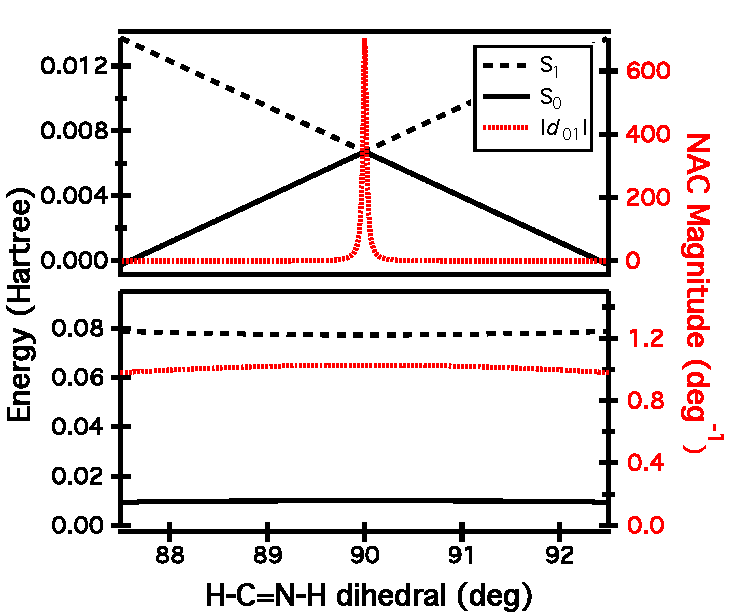
\includegraphics[width=\textwidth]{gs_es_dercp} 
  \caption{ }
  \label{fig:gs_es_dercp}
  \end{subfigure}
  \begin{subfigure}[b]{0.40\textwidth}
  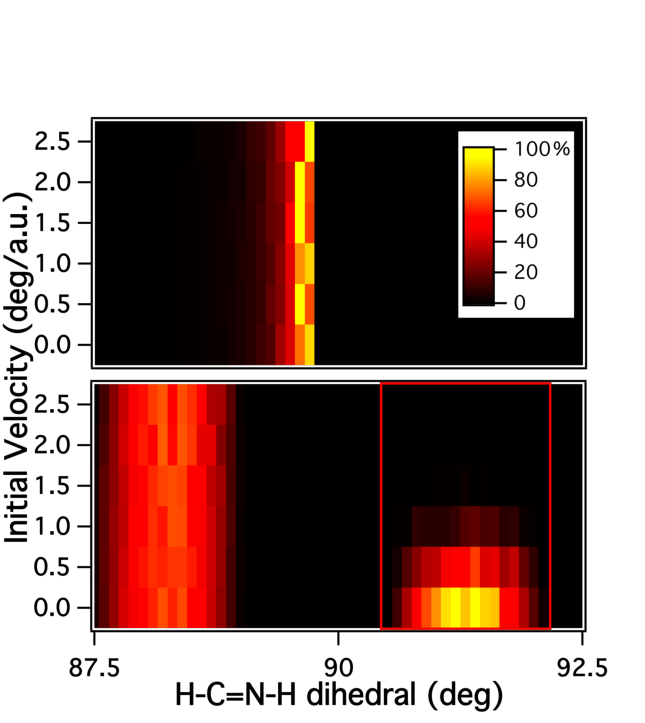
\includegraphics[width=\textwidth]{stacked_hops} 
  \caption{ }
  \label{fig:hops}
  \end{subfigure}
  \caption{\footnotesize (a) Potential energy surfaces for ground and excited
  states, and the coupling strength between the two states with respect to the
  dihedral angle in the vicinity of the minimum energy crossing point between
  S$_0$ and S$_1$ from the pp-TDA (top frame) and CIS (bottom frame) approaches.
  (b) Color maps showing the distribution of configurations at which hops from
  S$_1$ to S$_0$ occur for the different initial velocities resolved at the
  pp-TDA (top frame) and CIS (bottom frame) levels of theory (area in red box
  magnified, after normalization, 1000$\times$ for visibility.)}
\end{figure}

To demonstrate the performance of the pp-TDA within TSH over single reference
methods such as configuration interaction singles (CIS), we simulated the ground
state recovery dynamics for a small iminium ion, H$_2$C=NH$_2^+$, known to
readily photo-isomerize via a conical-intersection-mediated, non-radiative decay
from S$_1$ to the ground state, S$_0$, using both the CIS and pp-TDA description
of the adiabats. The important difference between the two methods is in an
asymmetric treatment of electron correlation in the ground and excited states in
the CIS, while the pp-TDA treats all of the states on the same footing. To
ensure that our dynamics simulation transversed the conical intersection, we
restricted the nuclear trajectories to the well--established isomerization
coordinate of the dihedral rotation.  Potential energy surfaces and coupling
strengths along the reaction coordinate are collected in \cref{fig:gs_es_dercp}. 
There are several conditions for determining the presence of a conical
intersection of PESs. A necessary and sufficient condition is the presence of a
degeneracy as well as a spike in the NAC magnitude in the neighborhood of the
proposed conical intersection (technically the NAC becomes undefined at the
conical intersection which exists at exactly one point on the PES).
It is clear to see that, via these conditions, the conical intersection along
the isomerization coordinate is not captured in the CIS PES, while the pp-TDA
exhibits the correct behavior.

10$^6$ TSH trajectories for a series of 6 initial velocities were considered for
each of the two electronic structure methods.  In all cases the electronic
superposition was initialized as a pure (S$_1$) state, and the dihedral angle
was chosen to be 87.5 degrees so that the dynamics are started in the upper
state near to the region of strongest coupling. Relation profiles for the S$_1$
to S$_0$ inter-conversion are given in the form of a heat plot in
\cref{fig:hops}. There are two characteristics of dynamics in the neighborhood
of conical intersections and are of interest in the relaxation
profiles\cite{Hynes14_97}. First of which is, if the conical intersection is
properly described, internal conversion from S$_1$ $\rightarrow$ S$_0$ should be
localized near the conical intersection. This feature is clearly captured by
the pp-TDA, while CIS suffers a broad relaxation profile that is qualitatively
incorrect. This incorrect profile is due to the artificially early onset of the
NAC along the isomerization coordinate which is a result of improper description
of the conical intersection. The second feature that is important to point out
is that, if the conical intersection is properly described, all of the classical
nuclear trajectories should interconvert before the conical intersection. This
feature is captured in the pp-TDA, even in the initial velocity limit. In the
CIS simulation, a small portion of the trajectories hop at configuration past
the conical intersection at the low initial velocity limit. This means that
those trajectories transversed the conical intersection throughout the
simulation. This qualitatively incorrect behavior would lead to
uncharacteristically long relaxation rates over the pp-TDA.

Although the pp-TDA has been shown to perform quite well in the proper treatment
of excited to ground state interconversion, its use as a general tool is quite
limited due to the presence of instabilities in the underlying reference
determinant throughout the dynamics simulation. The reason for this is the fact
that the reference determinant one that is optimized with respect to the ($N-2$)
cation of the molecular system. In the case of the iminum ion, the ground state
geometry is planar, while the conical intersection is located at the point where
diheral of the two functional groups is at 90 degrees. In the case of the
$N$-electron system, the ground state HF wave function is perfectly stable at
the ground state, while there exists a triplet instability in the singlet HF
wave function at the conical intersection. Interestingly, the exact opposite
problem occurs in the ($N-2$) electron system. This indicates a fundamental
problem in the single Slater determinantal wave function description of
molecular systems. One of the base assumptions of post SCF methods in electronic
structure is that the underlying reference determinant is stable at a given
molecular geometry. If that assumption is no longer valid, the behavior of
these methods often become ill defined. Thus it is important to utilize methods
that will ensure variational stability throughout the entire nuclear
configuration space.

